% Options for packages loaded elsewhere
\PassOptionsToPackage{unicode}{hyperref}
\PassOptionsToPackage{hyphens}{url}
%
\documentclass[
]{article}
\usepackage{amsmath,amssymb}
\usepackage{lmodern}
\usepackage{iftex}
\ifPDFTeX
  \usepackage[T1]{fontenc}
  \usepackage[utf8]{inputenc}
  \usepackage{textcomp} % provide euro and other symbols
\else % if luatex or xetex
  \usepackage{unicode-math}
  \defaultfontfeatures{Scale=MatchLowercase}
  \defaultfontfeatures[\rmfamily]{Ligatures=TeX,Scale=1}
\fi
% Use upquote if available, for straight quotes in verbatim environments
\IfFileExists{upquote.sty}{\usepackage{upquote}}{}
\IfFileExists{microtype.sty}{% use microtype if available
  \usepackage[]{microtype}
  \UseMicrotypeSet[protrusion]{basicmath} % disable protrusion for tt fonts
}{}
\makeatletter
\@ifundefined{KOMAClassName}{% if non-KOMA class
  \IfFileExists{parskip.sty}{%
    \usepackage{parskip}
  }{% else
    \setlength{\parindent}{0pt}
    \setlength{\parskip}{6pt plus 2pt minus 1pt}}
}{% if KOMA class
  \KOMAoptions{parskip=half}}
\makeatother
\usepackage{xcolor}
\usepackage[margin=1in]{geometry}
\usepackage{graphicx}
\makeatletter
\def\maxwidth{\ifdim\Gin@nat@width>\linewidth\linewidth\else\Gin@nat@width\fi}
\def\maxheight{\ifdim\Gin@nat@height>\textheight\textheight\else\Gin@nat@height\fi}
\makeatother
% Scale images if necessary, so that they will not overflow the page
% margins by default, and it is still possible to overwrite the defaults
% using explicit options in \includegraphics[width, height, ...]{}
\setkeys{Gin}{width=\maxwidth,height=\maxheight,keepaspectratio}
% Set default figure placement to htbp
\makeatletter
\def\fps@figure{htbp}
\makeatother
\setlength{\emergencystretch}{3em} % prevent overfull lines
\providecommand{\tightlist}{%
  \setlength{\itemsep}{0pt}\setlength{\parskip}{0pt}}
\setcounter{secnumdepth}{-\maxdimen} % remove section numbering
\ifLuaTeX
  \usepackage{selnolig}  % disable illegal ligatures
\fi
\IfFileExists{bookmark.sty}{\usepackage{bookmark}}{\usepackage{hyperref}}
\IfFileExists{xurl.sty}{\usepackage{xurl}}{} % add URL line breaks if available
\urlstyle{same} % disable monospaced font for URLs
\hypersetup{
  pdftitle={Project Report},
  pdfauthor={Denise Stefania Cammarota},
  hidelinks,
  pdfcreator={LaTeX via pandoc}}

\title{Project Report}
\usepackage{etoolbox}
\makeatletter
\providecommand{\subtitle}[1]{% add subtitle to \maketitle
  \apptocmd{\@title}{\par {\large #1 \par}}{}{}
}
\makeatother
\subtitle{Lagged Cross-correlations between COVID-19 cases in
Argentinian provinces during initial stages of propagation}
\author{Denise Stefania Cammarota}
\date{2022-08-18}

\begin{document}
\maketitle

\hypertarget{introduction}{%
\subsection{Introduction}\label{introduction}}

COVID-19 is a disease caused by the SARS-COV-2 virus, which belong to
the family of coronaviruses. Some of these viruses have been known in
the past for causing mild to severe respiratory diseases in humans and
cause small to medium sized epidemics. However, COVID-19 spread became
worldwide not too late after the first cases were detected in late 2019
in China. As a consequence, COVID-19 has been defined as a pandemic on
the 11th March 2020 by the World Health Organization (WHO). In
Argentina, the first imported COVID-19 case was detected on March 2020.
Even though initial cases were imported, community propagation of the
virus rapidly took over in all Argentinian provinces (which are
Argentina's administrative divisions, similar to states). It is
remarkable that this happened even though strong isolation measures were
put into place as early as the March 15th 2020. In this context, it is
interesting to investigate which were the relationships between the
provinces. That is, we want to quantify how primary cases in one place
caused secondary cases elsewhere. Intuitively, this would have to do
with some measure of connectiveness between provinces and better
connected provinces like CABA (Argentina's capital) would have a strong
influence in epidemiological dynamics. Furthermore, provinces where the
first imported cases were detected would also play important roles in
the propagation.

In the literature, several authors have had the idea of understanding
how the connectiveness between places has influenced spread of COVID-19.
Some of them have used methods in order to detect clusters of similar
incidence of the disease over time. Others have used well-established
administrative divisions (like countries, provinces or states) and have
tried to use different methods to correlate them. During my master
research, we decided to use a standard way of quantifying relationships
between epidemic time series: lagged cross-correlations between time
series of infected in Argentinian provinces. In particular, we focused
on time series spanning 2020, since propagation began to be influenced
by many more factors afterwards (like vaccination).

In this project, my goal is to calculate these lagged cross-correlations
using R and analyze these results. The main questions that I want to
tackle are which provinces have higher/lower correlations and lags, if
this makes sense intuitively and if provinces which acted as drivers of
epidemic propagation could be determined from this analyses.

\hypertarget{information-about-the-dataset}{%
\subsection{Information about the
dataset}\label{information-about-the-dataset}}

The dataset that was used contains information on all tests performed on
a national scale. It was downloaded from the official website of the
Argentinian Ministry of Health, which is responsible for reporting tests
and cases across the country. This website is periodically updated to
include newer reports. In particular, the dataset we used for this study
was downloaded on August 13th of 2022 and contains tests up until the
second week of August of the same year. Since this dataset is
overwritten every time an update happens, I downloaded an uploaded it
\href{https://drive.google.com/file/d/1j1QXQZu60LGApLWroKqafhmUa9XdE-m7/view?usp=sharing}{on
this link} of my personal Drive. Total size of the dataset is about 6GB.

This dataset has several attributes for each record, of which we are
interested by the following 4: - residencia\_provincia\_nombre: name of
the province of the corresponding record. - clasificacion\_resumen:
tells whether a record corresponds to a confirmed, suspected, discarted
or probable case. - fecha\_inicio\_sintomas: date of symptom onset, as
informed by the patient. - fecha\_apertura: date the report of a record
on the system.

\hypertarget{data-exploring}{%
\subsection{Data Exploring}\label{data-exploring}}

The data is explored on the \texttt{1\_explore\_cases.R} of the
\texttt{R} folder of the project. First, the data is uploaded using the
function \texttt{fread} of the \texttt{data.table} library, which
supports the reading of large files. After importing, we identify
possible values for all values of interest. Firstly,
\texttt{residencia\_provincia\_nombre} can take on all names of the 24
Argentinian provinces plus an unspecified value coined
\texttt{SIN\ ESPECIFICAR} when the province is not specified in the
offical database. Secondly, \texttt{clasificacion\_resumen} can be:
Confirmado, Descartado, Probable or Sospechado. Regarding dates, if we
filter for 2020 reports, both \texttt{fecha\_inicio\_sintomas} and
\texttt{fecha\_apertura} can take on all values between January 1st 2020
and December 31st 2020. It is important to remark that NA values can be
found in the \texttt{fecha\_inicio\_sintomas} column.

Since no NAs can be found in \texttt{fecha\_apertura}, it is interesting
to investigate the relationship between this date and the date of first
symptom onset. This can give us some hints on how to replace missing
\texttt{fecha\_inicio\_sintomas} values. This is done in the following
plot, which represents an histogram of the difference
\texttt{fecha\_apertura\ -\ fecha\_inicio\_sintomas}, measured in days.
Furthermore, we plot the mean of this difference as well as the interval
defined by its standard deviation.

\begin{figure}
\centering
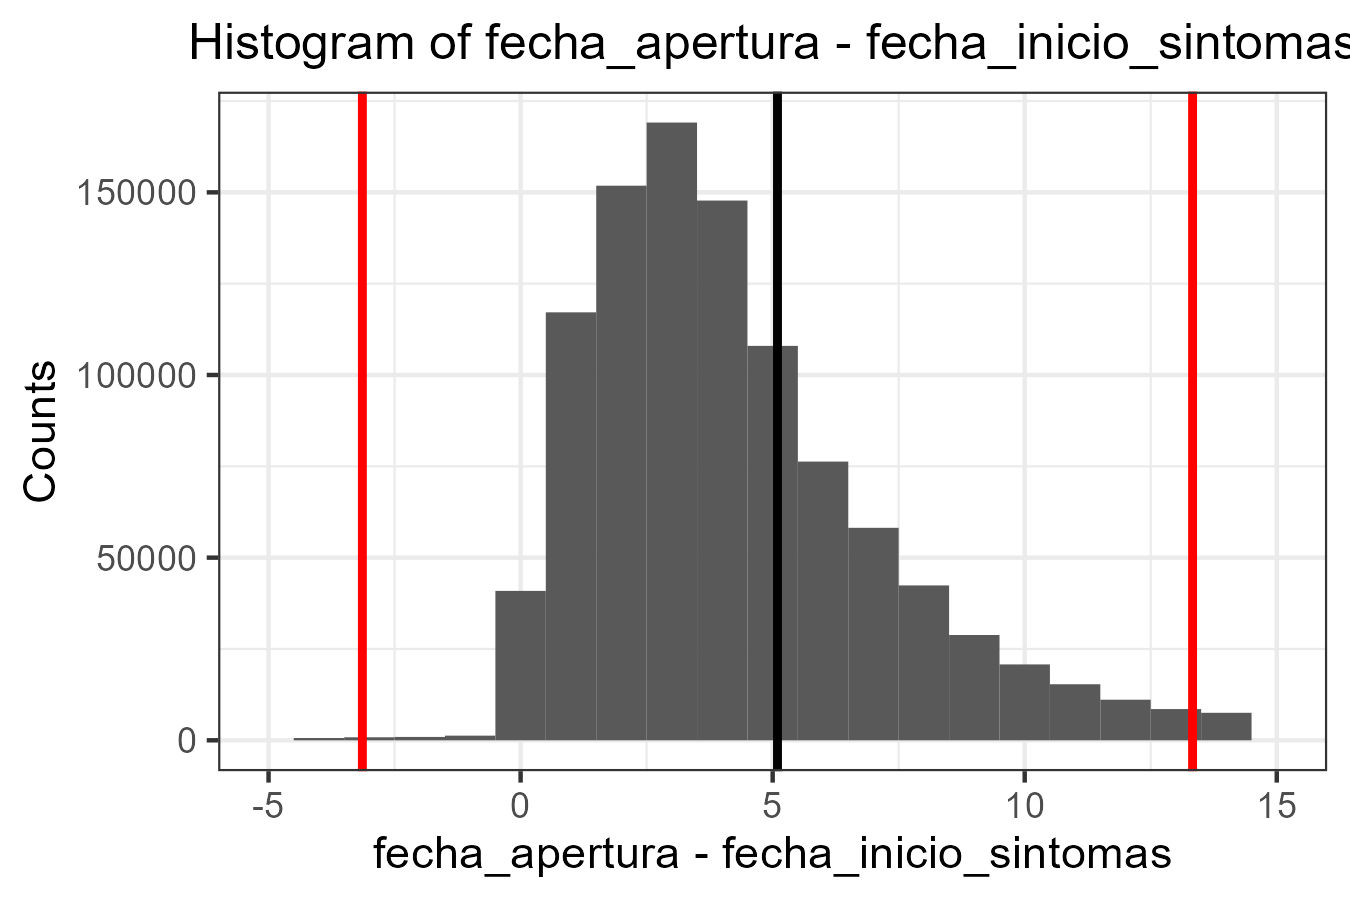
\includegraphics[width=0.5\textwidth,height=\textheight]{../figs/dates_diff.png}
\caption{Histogram of difference between date of report and date of
symptom onset.}
\end{figure}

Here, we can observe that the distribution of differences is not
symmetric. That is, the date of report in the system is usually later
than the date of symptom onset, which makes intuitive sense. The mean of
this distribution is about 5 days, whereas the mean is approximately 8
days.

\hypertarget{data-processing}{%
\subsection{Data Processing}\label{data-processing}}

The data is processed in script \texttt{2\_process\_data.R}. Firstly, it
is loaded in a similar manner as in the previous script of our workflow.
Then, we apply a filter to get confirmed cases with
\texttt{clasificacion\_resumen\ =\ Confirmado} and with report and
symptom onset dates in 2020. Since some values of
\texttt{fecha\_inicio\_sintomas} are missing, we replace them by a
random date in between the corresponding reporting date and 8 days
before. This was the standard used in my group during my thesis.
However, upon looking at the plot from the previous section, some
modifications could be made.

Once there are no NAs present, script \texttt{3\_get\_tseries\_cases.R}
obtains the time series of new cases per day by province and arranges
them in a 24 x 365 matrix. This makes sense since there are 24 provinces
and 365 days in 2020. Finally, we sum dates every 14 days using external
function \texttt{get\_infected}. This gives us time series of estimated
infected by province, since initially the contagious period (and
therefore, the imposed isolation period) was estimated to be 14 days.
Processed data are saved in file \texttt{cases\_processed.csv} of
\texttt{data/raw} folder.

As a result, we save this matrix of infected per day per province in
file \texttt{cases\_provs.csv}, along with two extra files: one
\texttt{cases\_names\_provs.csv} containing the order of provinces
within the matrix and one \texttt{cases\_dates\_provs.csv} containing
the order of dates. All this files can be found in the \texttt{outputs}
folder of the project.

\hypertarget{computing-correlations-and-lags}{%
\subsection{Computing Correlations and
Lags}\label{computing-correlations-and-lags}}

The \texttt{4\_compute\_corr\_cases.R} script is dedicated to the
calculations of the actual lags and correlations between time series
using the outputs generated in the last section. In order to calculate
this quantities, we use the function \texttt{lagged\_correlations.R}
which receives the matrix of the time series and returns two matrices:
one for the lags and one for correlations.

This function does two loops to obtain every possible combination of
pairs of provinces. For each pair, it calculates correlations by
shifting one series with respect to the other by a number of days.
Afterwards, it defines the lag between provinces as the shift in days
for which correlation is maximum, and that maximum correlation as the
actual correlation.

The results of this script, the correlation and lags matrices, are saved
\texttt{outputs} folder in files \texttt{cases\_corrs\_provs.csv} and
\texttt{cases\_lags\_provs.csv} respectively.

\hypertarget{analysis-of-results}{%
\subsection{Analysis of results}\label{analysis-of-results}}

\hypertarget{correlations-between-provinces}{%
\subsubsection{Correlations between
provinces}\label{correlations-between-provinces}}

\begin{figure}[h]
\begin{subfigure}{.5\textwidth}
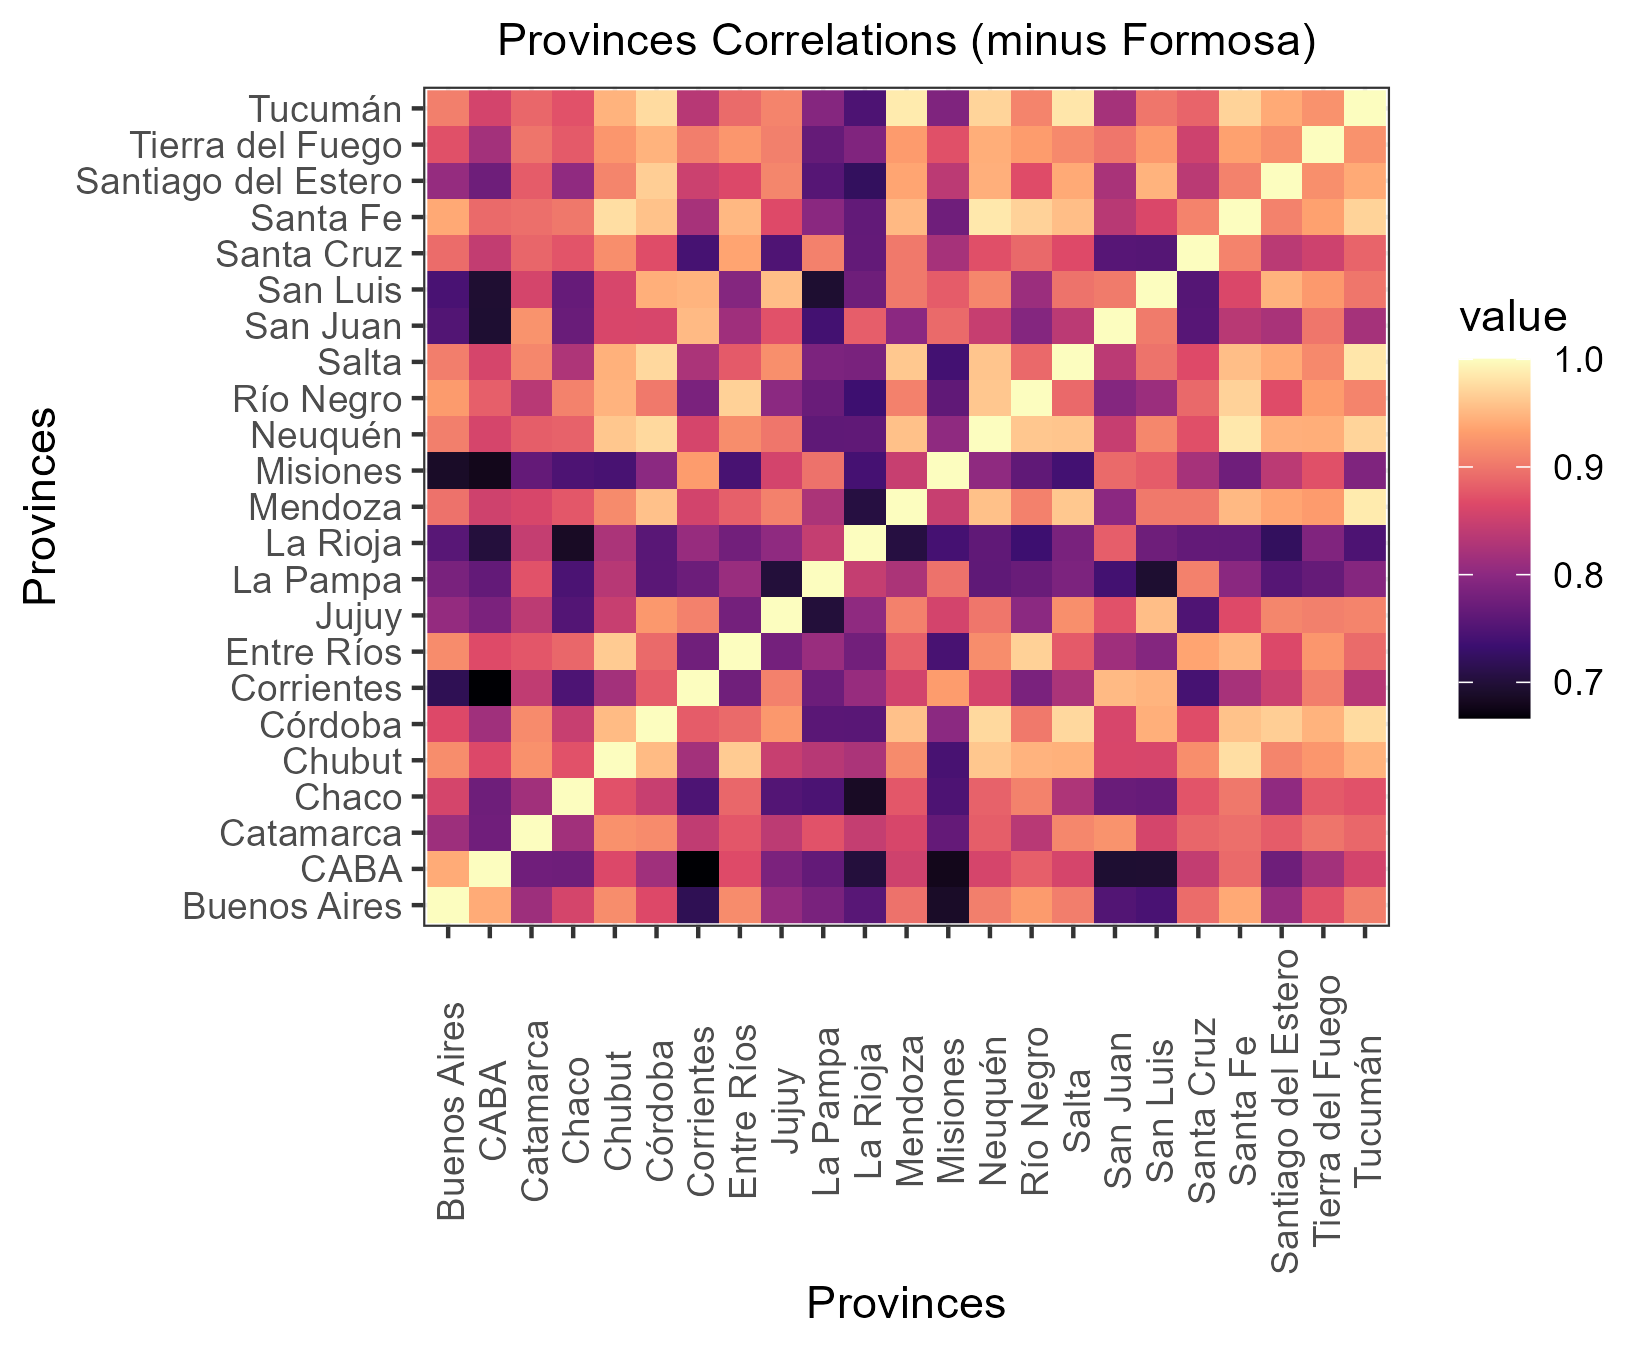
\includegraphics[]{fig/cases_corrs_sf.png}
\end{subfigure}%
\begin{subfigure}{.5\textwidth}
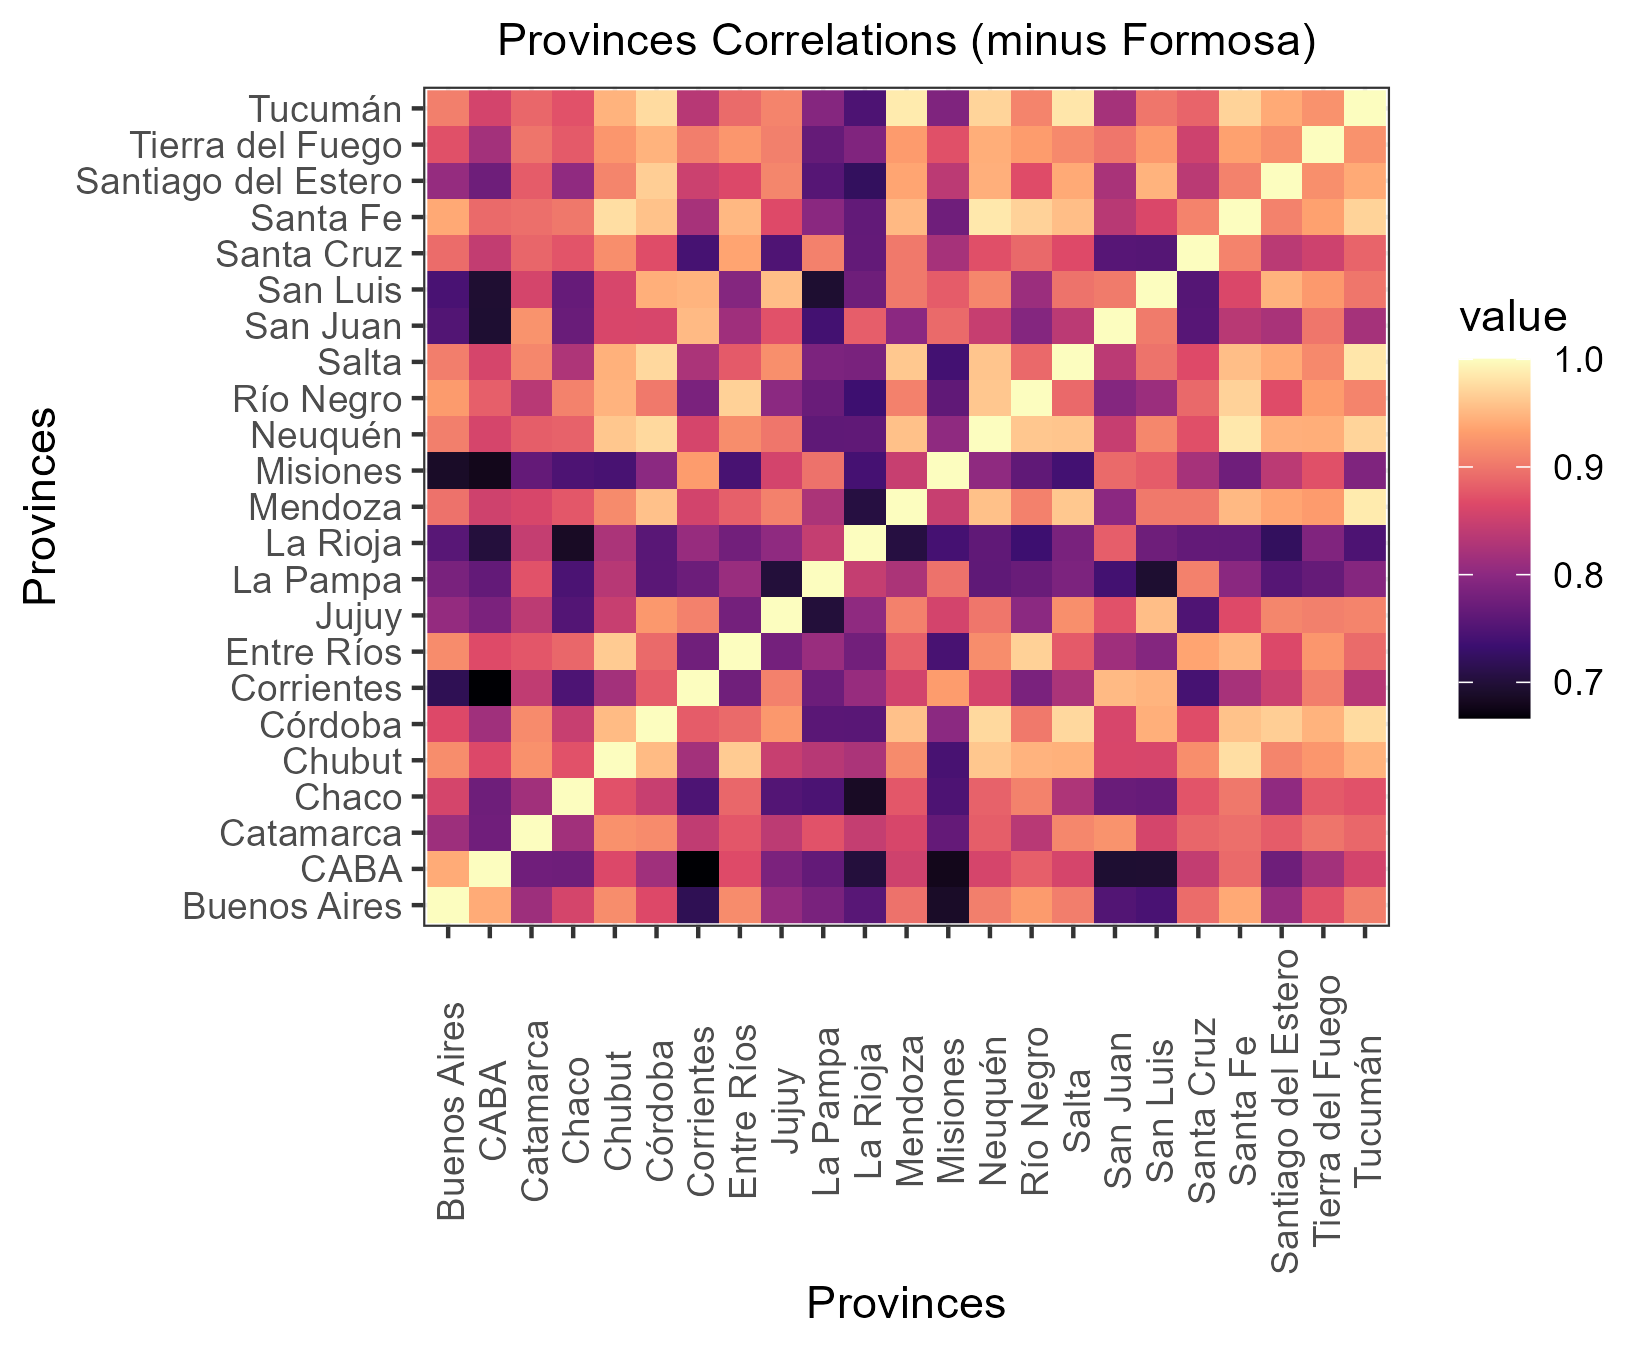
\includegraphics[]{fig/cases_corrs_sf.png}
\end{subfigure}
\caption{caption}
\end{figure}

\hypertarget{lags-between-provinces}{%
\subsubsection{Lags between provinces}\label{lags-between-provinces}}

\hypertarget{references}{%
\subsection{References}\label{references}}

\end{document}
